\chapter*{Conclusioni e sviluppi futuri}
\addcontentsline{toc}{chapter}{Conclusioni e sviluppi futuri}
\markboth{Conclusioni e sviluppi futuri}{Conclusioni e sviluppi futuri}

Nel campo dell'\textit{image processing} e del riconoscimento ottico dei caratteri (\textit{OCR}) risulta difficile produrre risultati accurati in modo efficiente. Lo studio degli algoritmi descritti in questa tesi ha permesso l'implementazione di svariate soluzioni per apportare migliorie della libreria QIOCR in termini di correttezza e velocit\`a di esecuzione.\par
\begin{wrapfigure}{L}{0.35\textwidth}
	\centering
	\frame{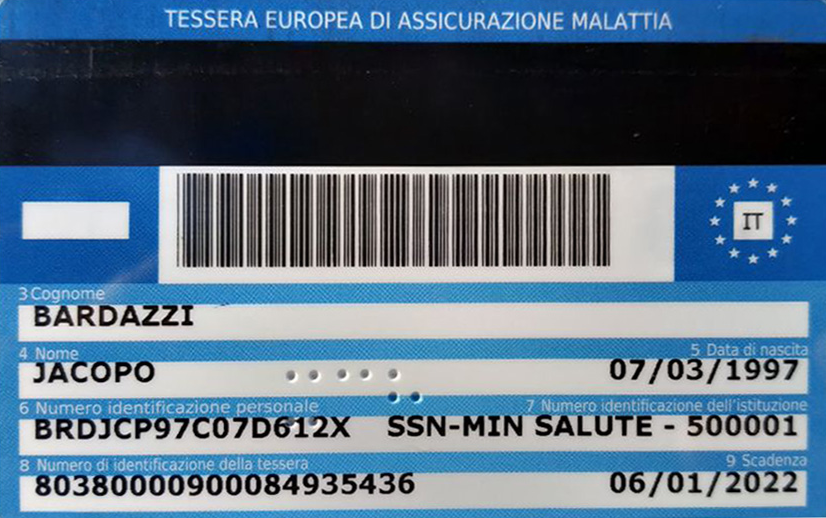
\includegraphics[width=0.28\textwidth]{img/ts-r-example.png}}
	\caption{Tessera sanitaria retro con \textit{barcode}} \label{fig:ts-r-example}
\end{wrapfigure}
Con il lavoro svolto, siamo riusciti a incrementare notevolmente la percentuale di campi esattamente uguali ai valori direttamente osservabili, passando da un'accuratezza del 5\% a una pari a circa il 70\% sul numero totale di campi processati, che sono solo alcuni dei campi dei documenti d'identit\`a supportati. 
Per esempio, per la \textit{tessera sanitaria retro} (vedi figura \ref{fig:ts-r-example}) viene considerato solamente il \textit{codice fiscale}, mentre per la \textit{carta d'identit\`a fronte} si considerano \textit{nome}, \textit{cognome} e \textit{data di nascita}. Nel caso di pi\`u campi il risultato passa il controllo solo se tutti rispettano l'uguaglianza con il dato effettivo.\par 
I tempi di esecuzione variano dai 5 ai 10 secondi per documento, a seconda della possibile difficolt\`a nelle operazioni di \textit{image matching}. In particolare, riusciamo a ottenere i risultati migliori nel caso in cui l'immagine analizzata sia una scansione, oppure quando questa \`e una fotografia scattata in modo parallelo rispetto al documento inquadrato.\par
\begin{wrapfigure}{R}{0.35\textwidth}
	\centering
	\frame{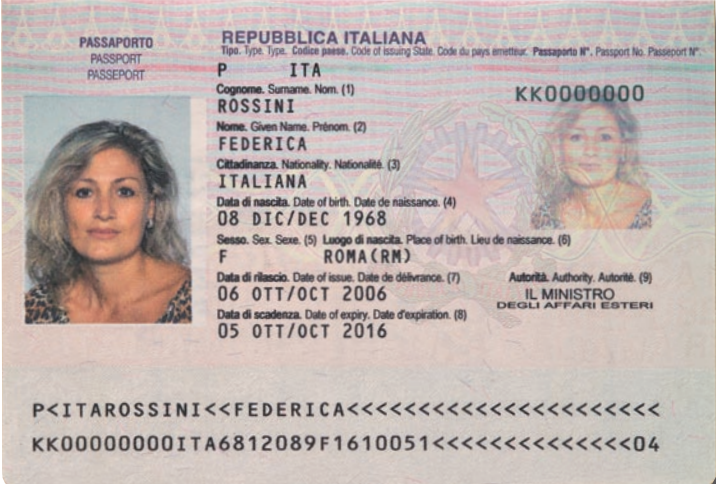
\includegraphics[width=0.28\textwidth]{img/passport.png}}
	\caption[Passaporto italiano con \textit{MRZ}]{Passaporto italiano con \textit{MRZ}\protect\footnotemark} \label{fig:passport}
\end{wrapfigure}
\footnotetext{\textit{Fonte}: \url{http://www.esteri.it/mae/doc/specifiche_pass_italiani.pdf}}
Per quanto riguarda il futuro, si ipotizza l'implementazione di nuovi documenti, quali il passaporto italiano (vedi figura \ref{fig:passport}), e si prevede l'aggiunta di nuove funzioni, come la lettura di codici a barre e di \textit{MRZ} (\textit{Machine Readable Zone}). Inoltre, si considera il supporto di documenti d'identit\`a di altri paesi europei, in modo da poter estendere il mercato d'interesse del prodotto.\par
L'utilizzo della libreria \`e stato venduto ad alcuni clienti dell'azienda, che sfruttano tuttora le funzionalit\`a offerte.
